% Likelihood scans with nuisance groups without the FSR cut
The extraction of the signal strength modifier $\mu$ proceeds through the maximisation of the likelihood,
as described in Section~\ref{sec:statistical_analysis}.
This procedure can be visualised by scanning the likelihood function for several values of the parameter $\mu$ while profiling the nuisance parameters.
For each value the best fit value of the nuisance parameters is computed,
and the resulting value of the likelihood is stored.
These points are then plotted as a function of $\mu$.

Usually the auxiliary quantity $-2\Delta\text{ln}\Likelihood$ (defined as $t_0$ in Equation~\ref{eq:test_statistic})
is used instead of the likelihood itself.
The width of the its profile is linked to the uncertainty on the estimate of $\mu$ from the fit.
More precisely, the set of values $\{ \mu / -2\Delta\text{ln}\Likelihood(\mu) < 1 (4) \}$ corresponds to the 68\usep\% (95\usep\%) confidence interval.

This procedure can also be performed by fixing the values of one or more nuisances instead of allowing them to be fitted by the algorithm.
The effect of fixing the value of one or more parameters is a reduction in the width of the likelihood shape.
This difference is ascribed to the effect of the frozen parameters.

Four groups of parameters are used in the following results:
\begin{itemize}
\item \textbf{theory:} uncertainties on the QCD scale, proton PDFs and on the value of \alpS;
\item \textbf{data-driven:} uncertainties related to the data-driven estimate of fake lepton or fake photon backgrounds;
\item \textbf{luminosity:} the uncertainty on the integrated luminosity corresponding to the data collected by the CMS experiment;
\item \textbf{others:} remaining experimental uncertainties, such as the lepton or photon efficiency scale factors or the \pileup weight;
\end{itemize}

\todo{describe results}

\newcommand{\descriptionFakePhoton}[1]{\if d#1%
The data-driven estimate for \nonprompt photons is used%
\else
\Nonprompt photons are estimated from simulation%
\fi}

\newcommand{\captionScan}[5]{
Likelihood scan for the signal strength parameter
on the #1,
using the #2 working point of the photon #3.
\descriptionFakePhoton{#4}.
The FSR cut is #5 applied.
The effect of groups of nuisance parameters on the uncertainty is assessed by sequentially fixing their value in the fit.
}

\begin{figure}
  \centering
  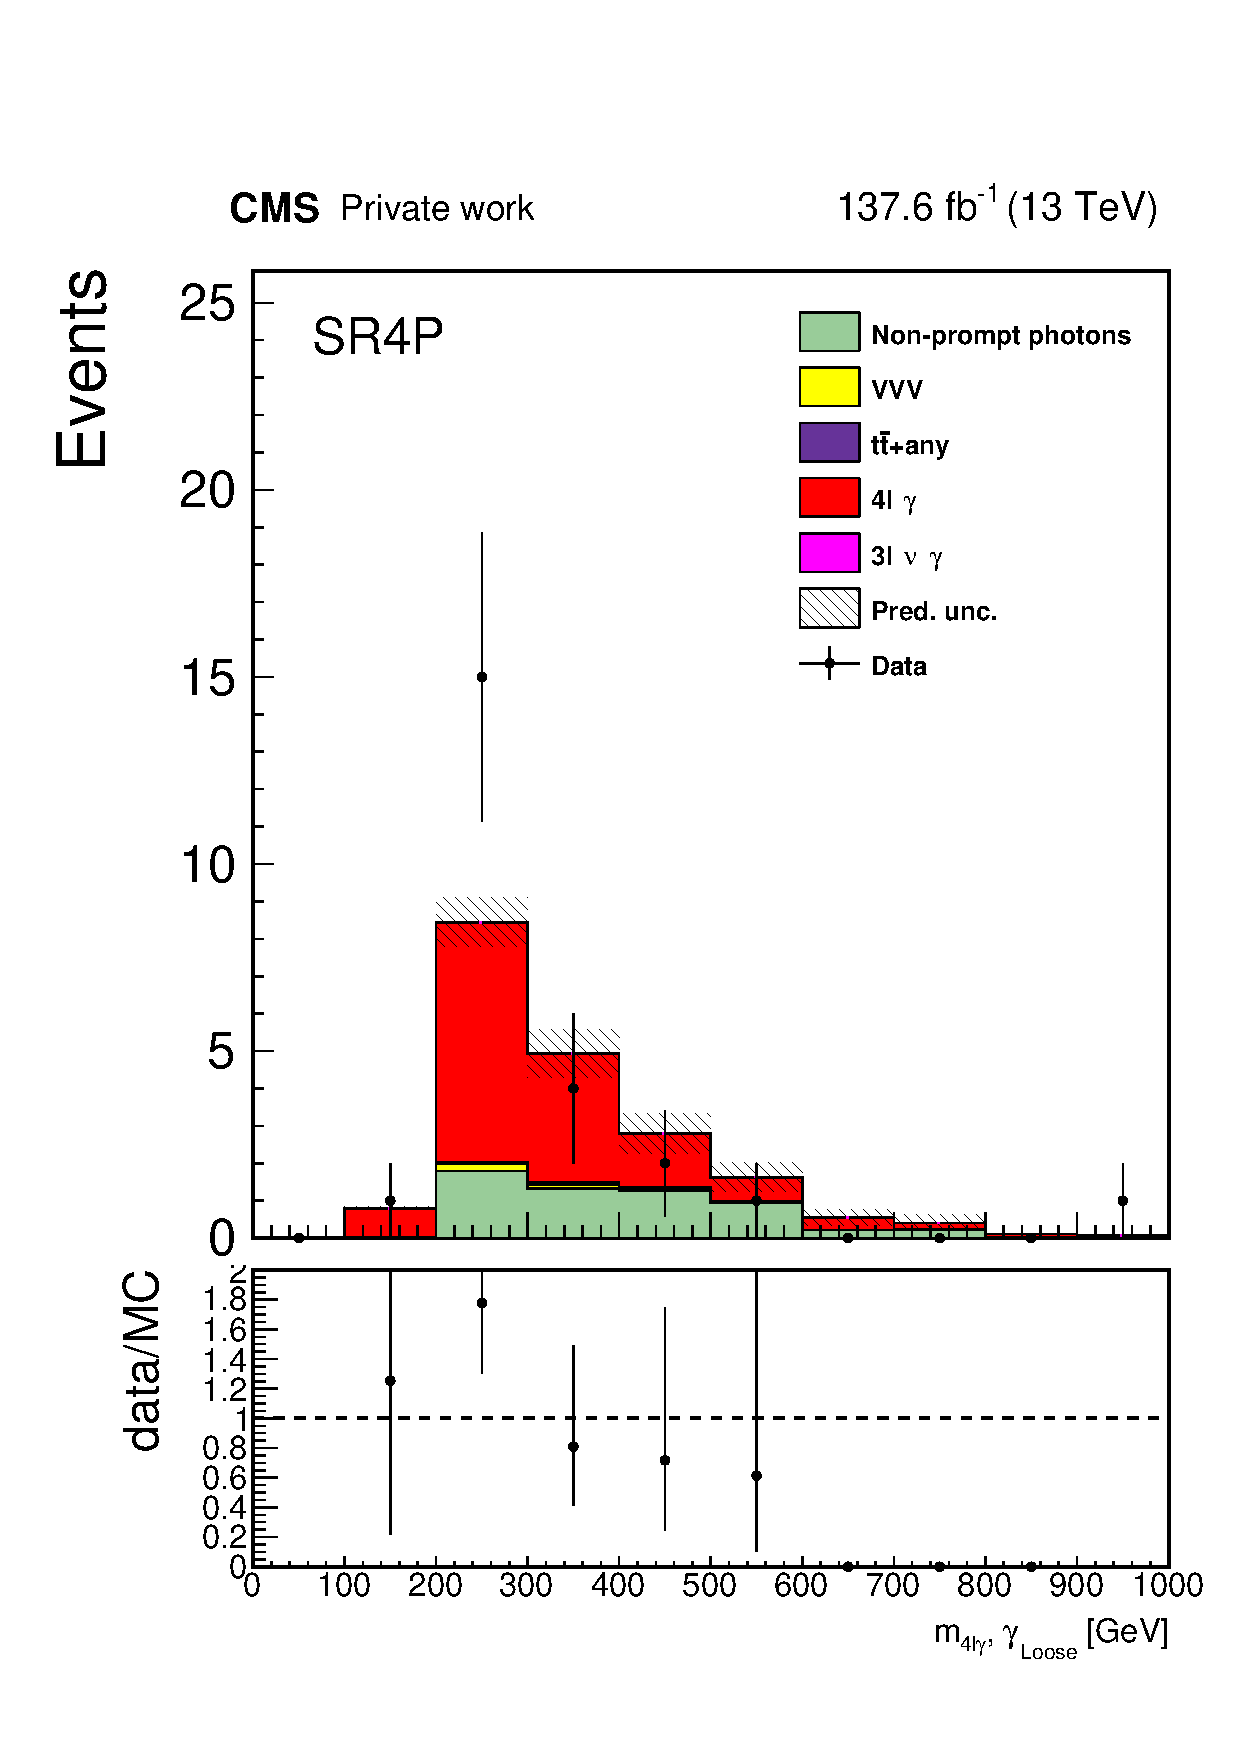
\includegraphics[height=.33\textheight]{Figures/dataMC/Run2/phoCR/SR4P/SYS_mZZGloose_central_pow.pdf}
  \hfill
  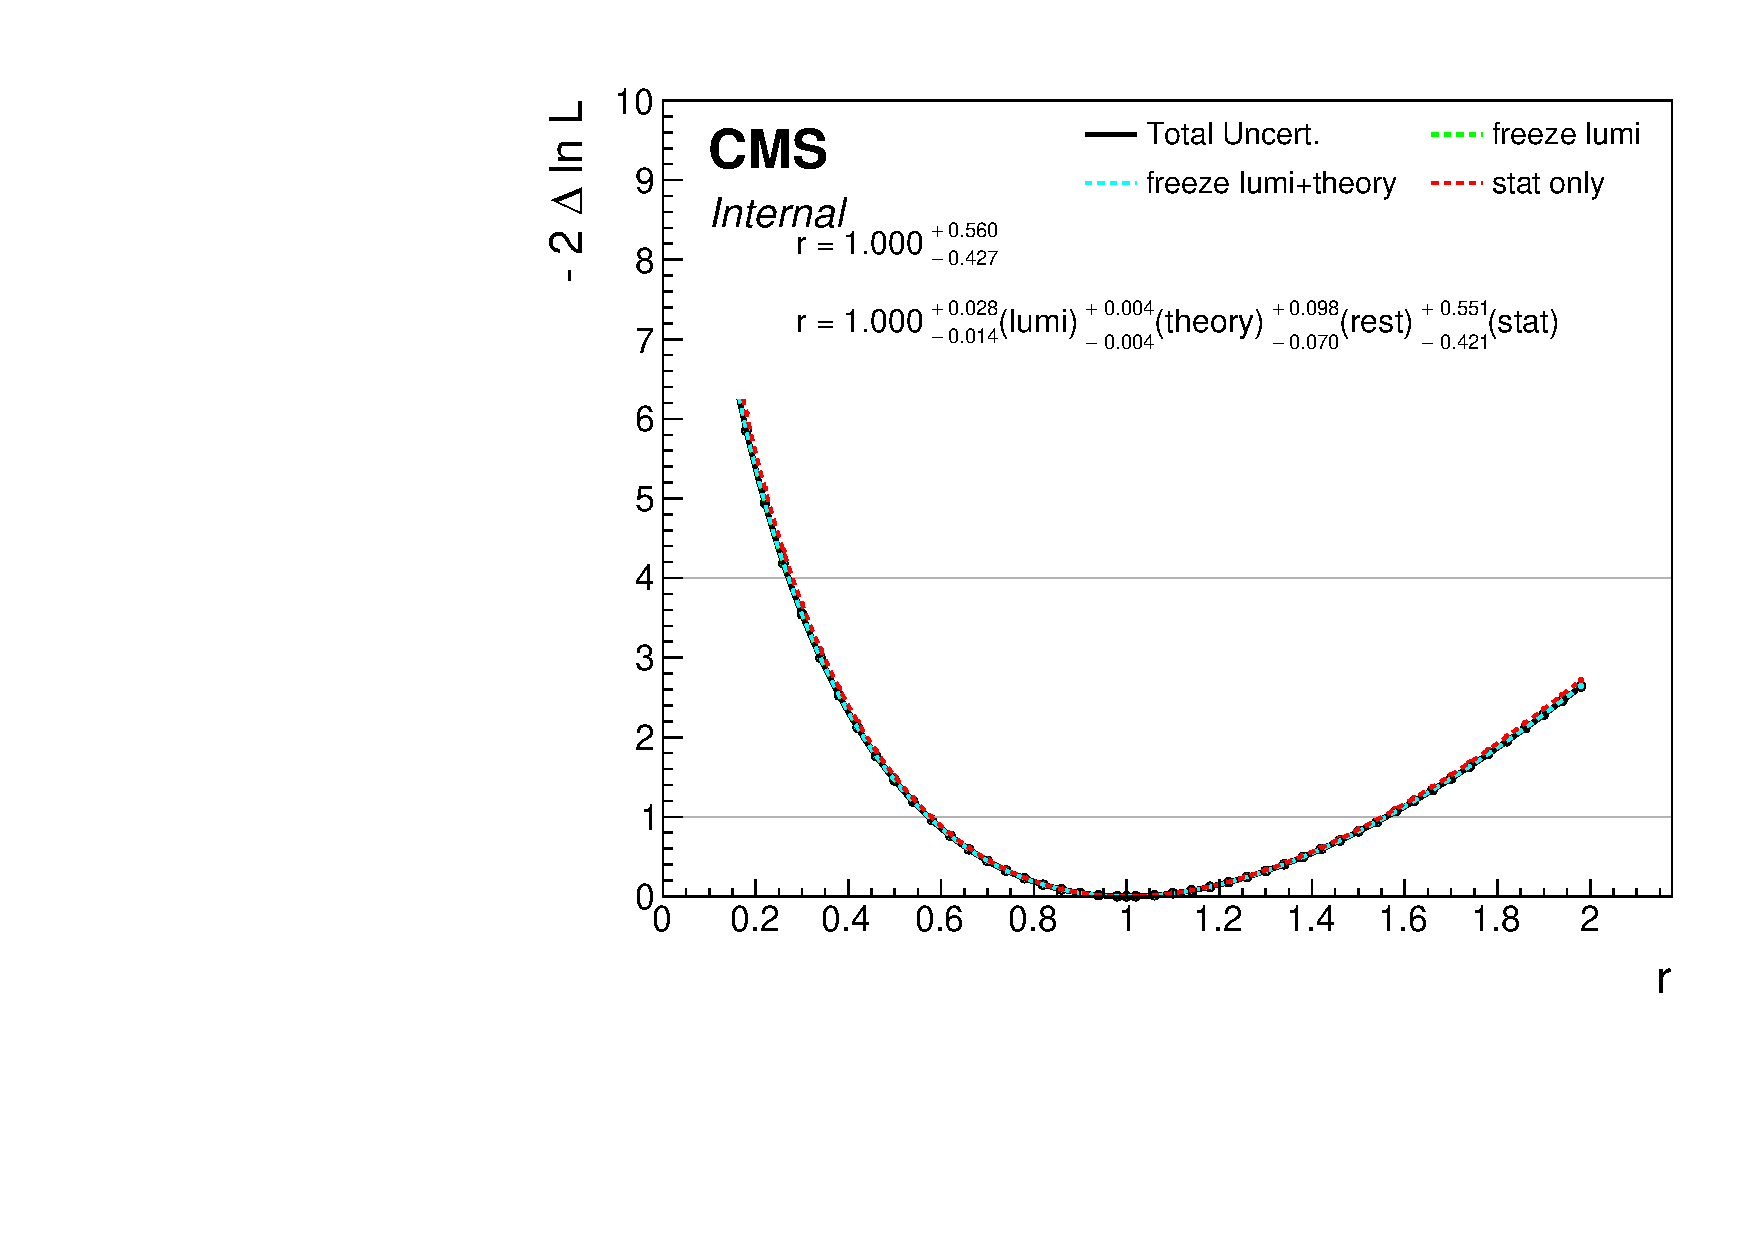
\includegraphics[height=.33\textheight]{scan_expected_Run2_SR4P_phoCR_lepCR_mZZGloose.pdf}
  \caption{\captionScan{mass of the $\PZ\PZ\PGg$ system}{Loose}{cut-based ID}{d}{}}
  \label{fig:scan_Run2_SR4P_phoCR_lepCR_mZZGloose}
\end{figure}

\begin{figure}
  \centering
  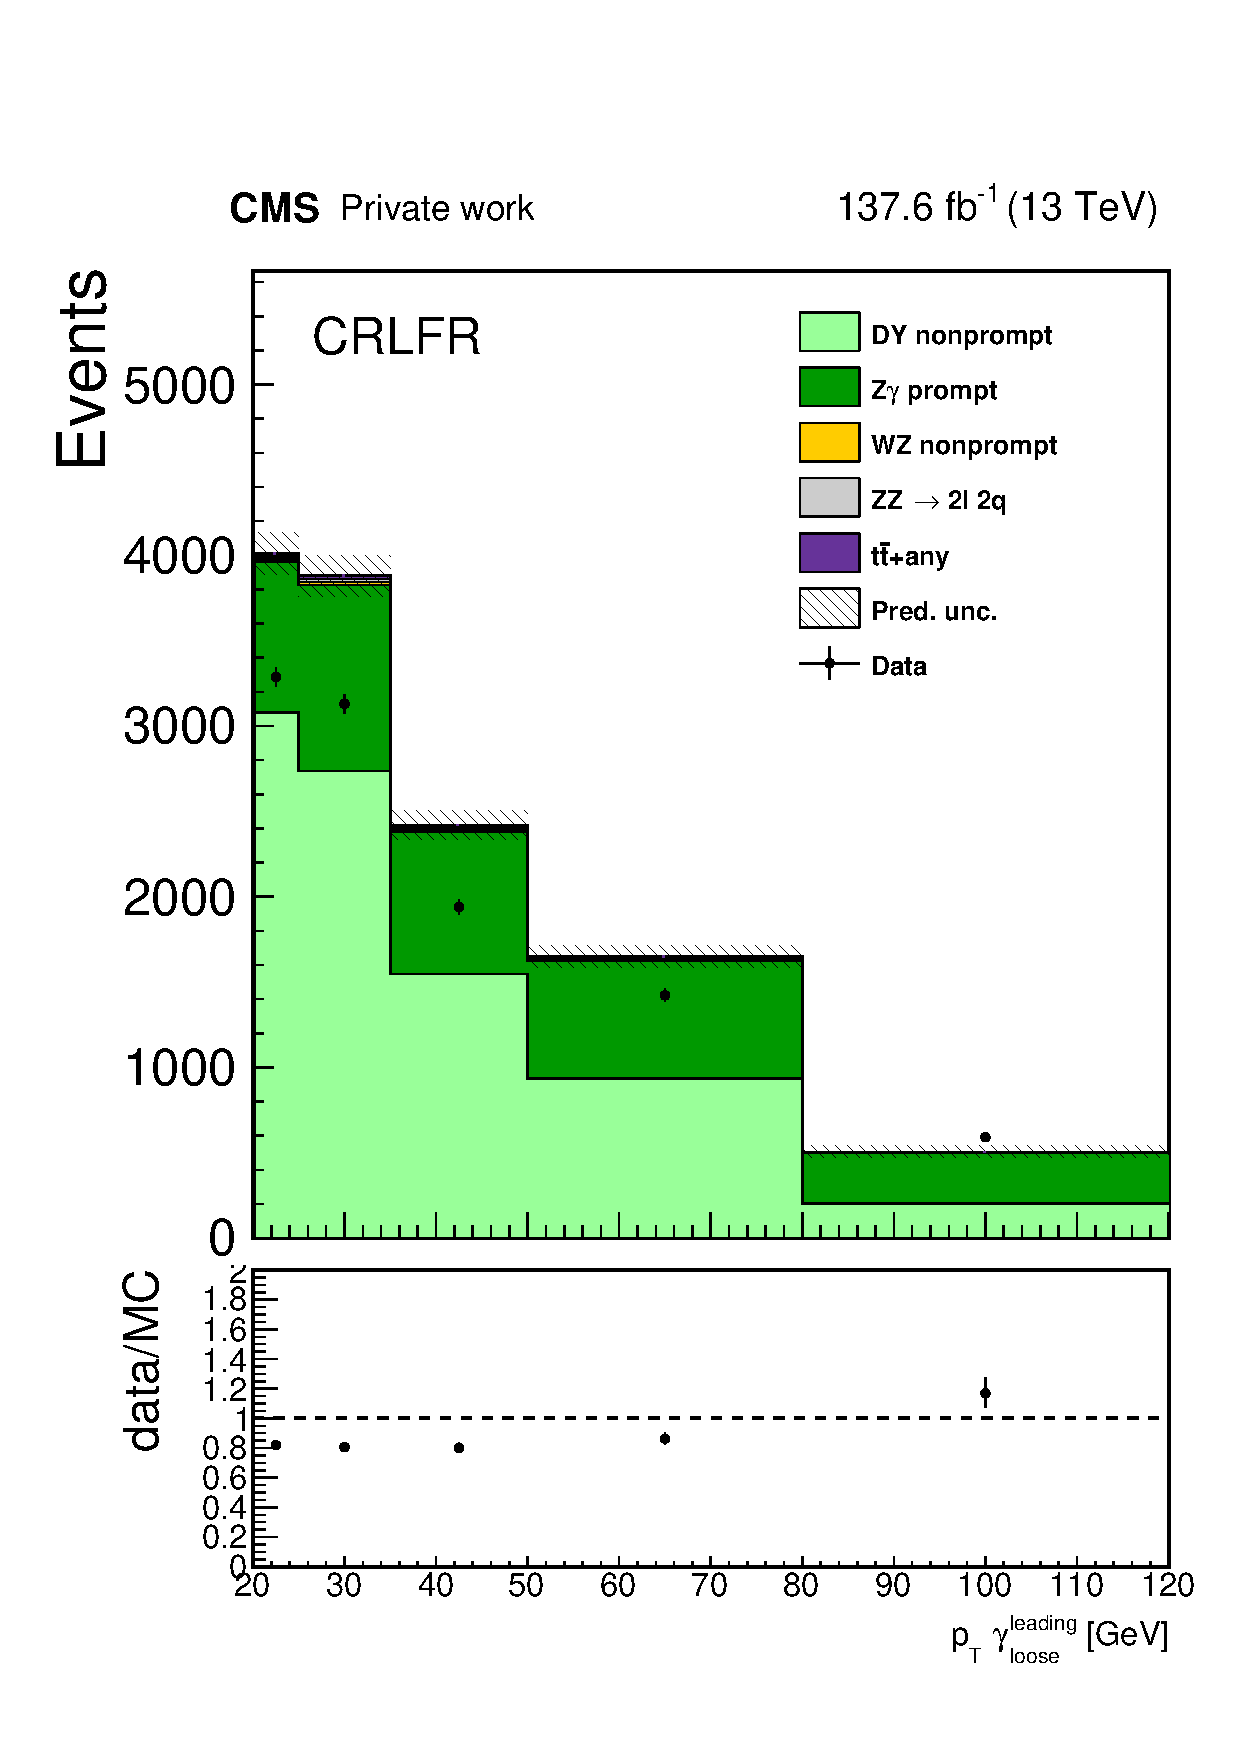
\includegraphics[height=.33\textheight]{Figures/dataMC/Run2/lepCR/SR4P/lead_loose_pt_pow.pdf}
  \hfill
  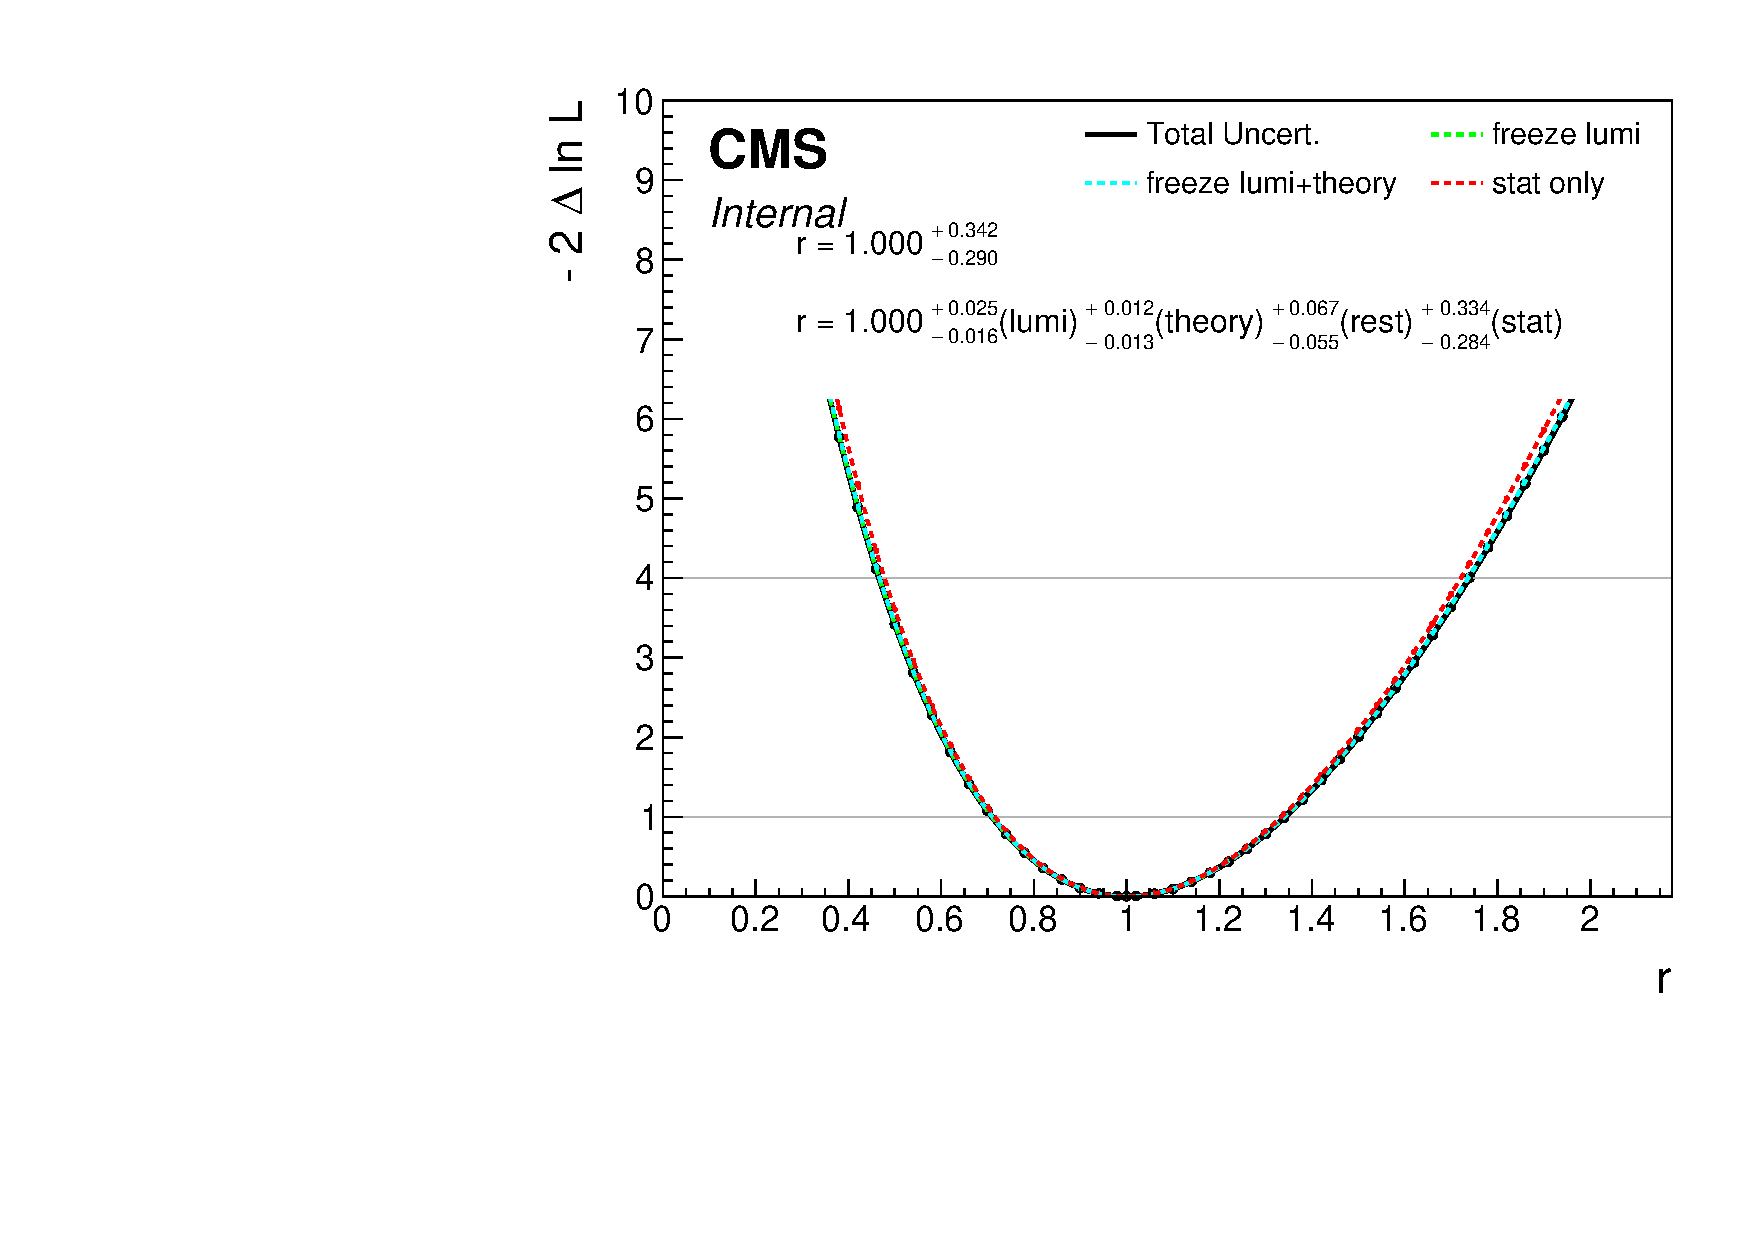
\includegraphics[height=.33\textheight]{scan_expected_Run2_SR4P_phoMC_lepCR_mZZGloose.pdf}
  \caption{\captionScan{mass of the $\PZ\PZ\PGg$ system}{Loose}{cut-based ID}{s}{}}
  \label{fig:scan_Run2_SR4P_phoMC_lepCR_mZZGloose}
\end{figure}

\begin{figure}
  \centering
  \includegraphics[height=0.33\textheight]{Figures/dataMC/Run2/lepCR/SR4P/SYS_mZZGwp90_central_pow.pdf}
  \hfill
  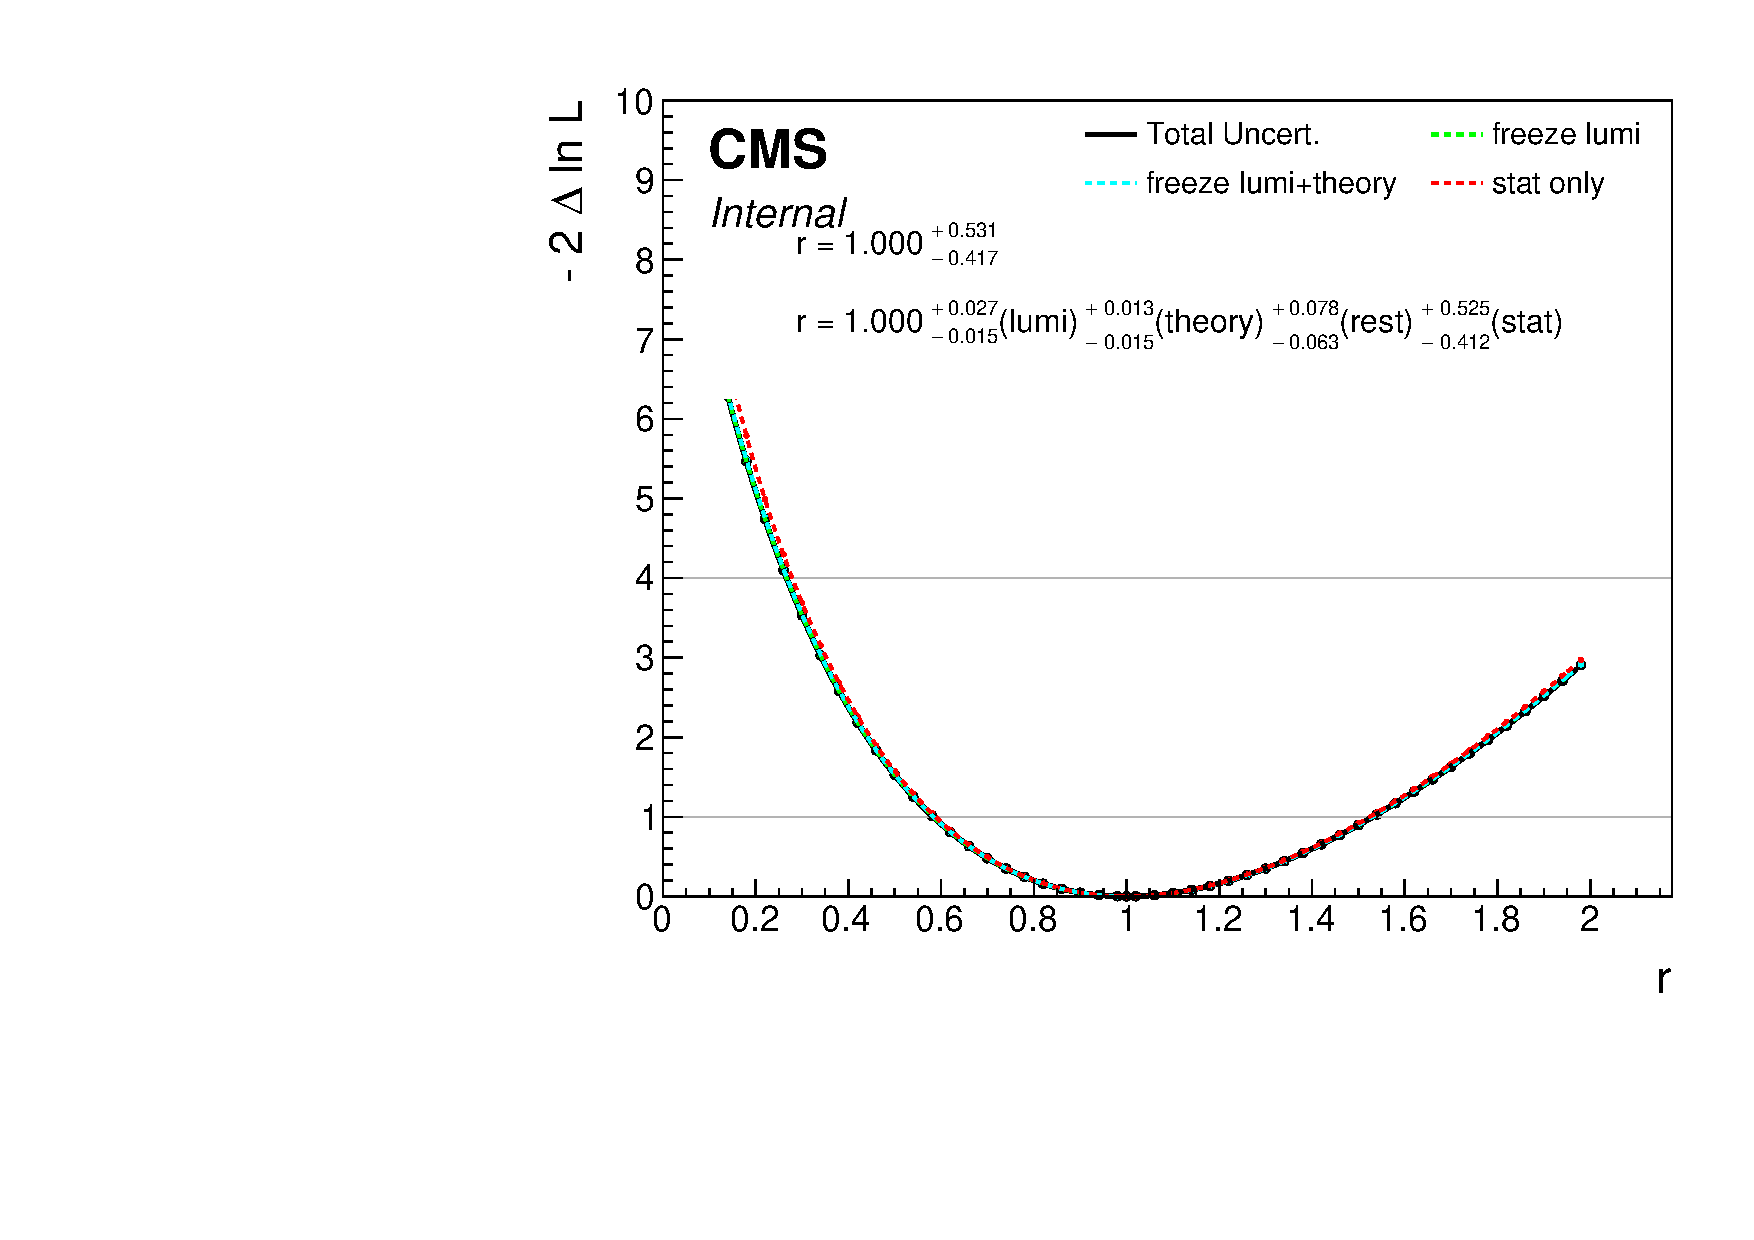
\includegraphics[height=.33\textheight]{scan_expected_Run2_SR4P_phoMC_lepCR_mZZGwp90.pdf}
  \caption{\captionScan{mass of the $\PZ\PZ\PGg$ system}{\texttt{wp90}}{MVA ID}{s}{}}
  \label{fig:scan_Run2_SR4P_phoMC_lepCR_mZZGwp90}
\end{figure}

\begin{figure}
  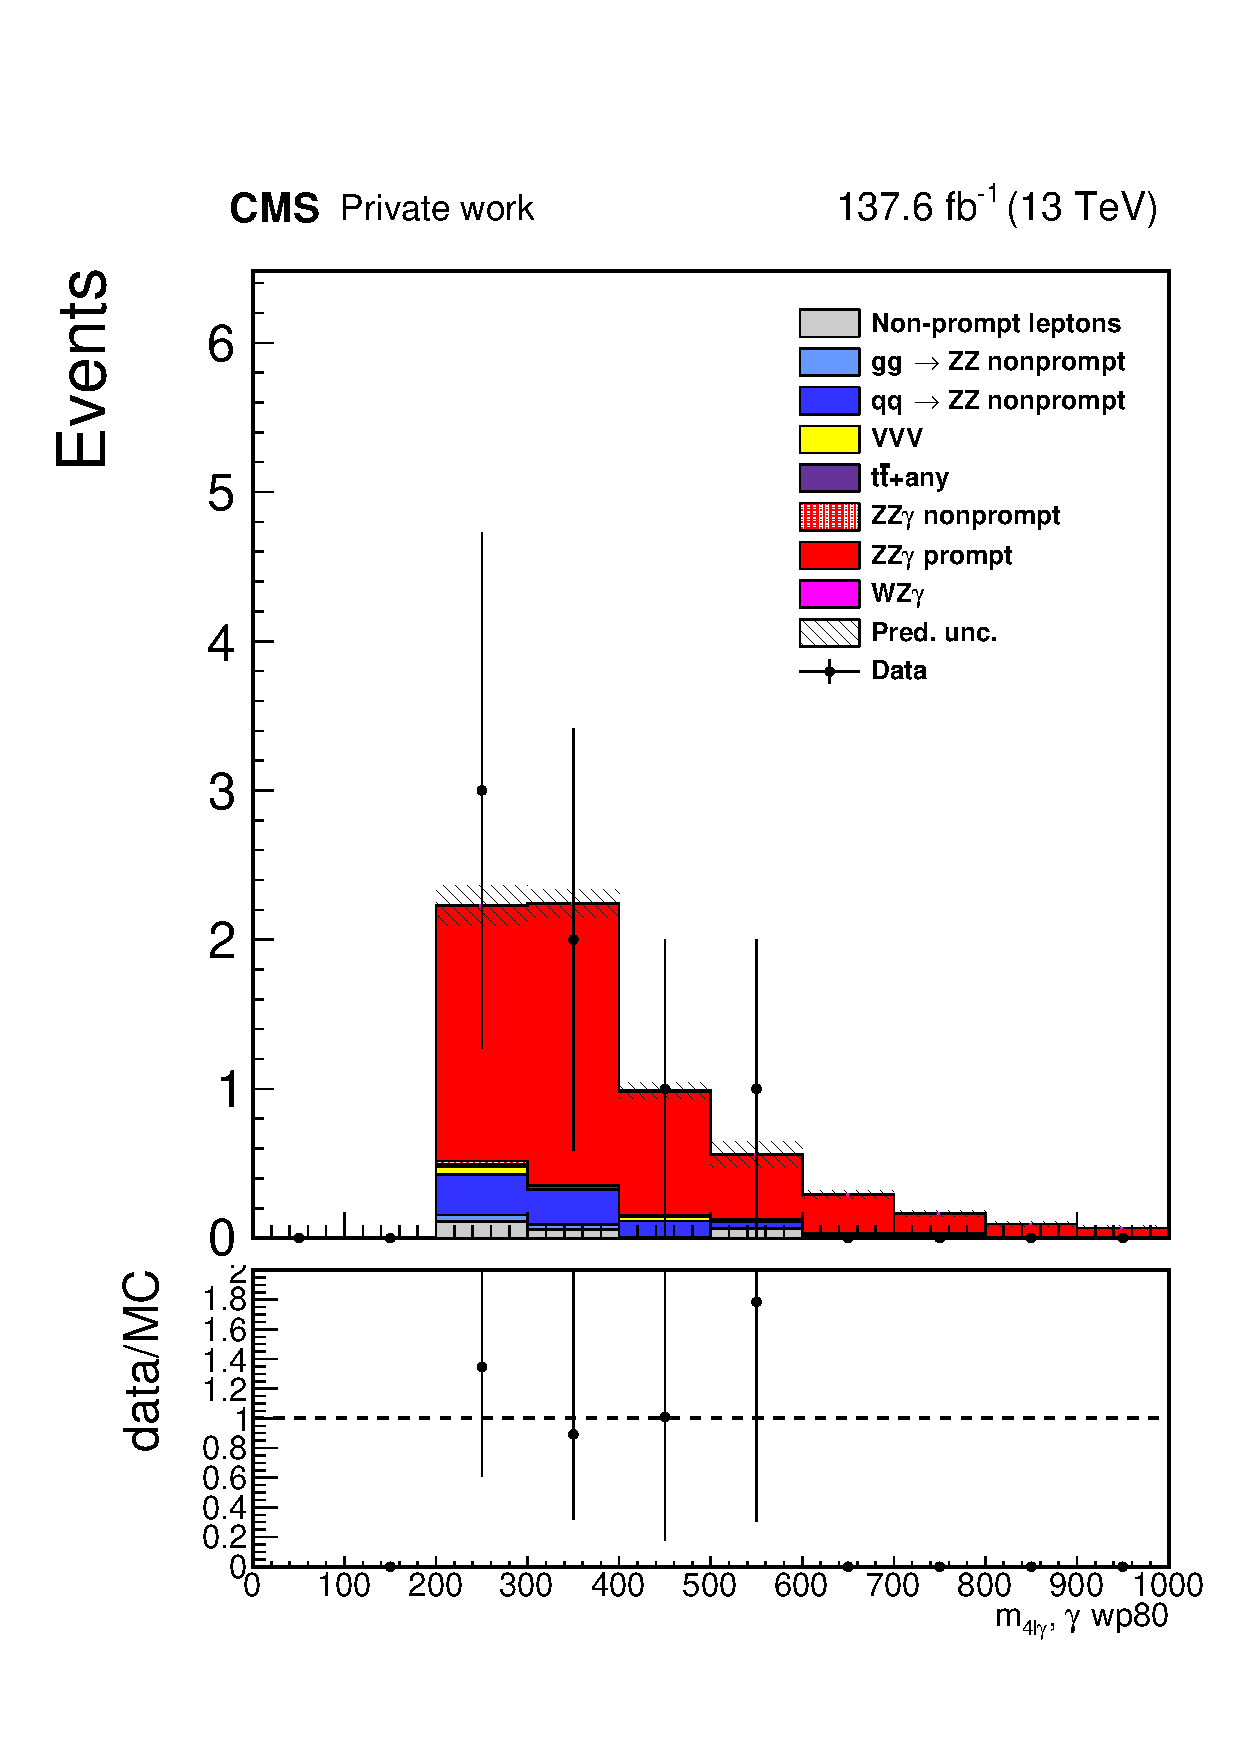
\includegraphics[height=0.33\textheight]{Figures/dataMC/Run2/lepCR/SR4P/SYS_mZZGwp80_central_pow.pdf}
  \hfill
  \centering
  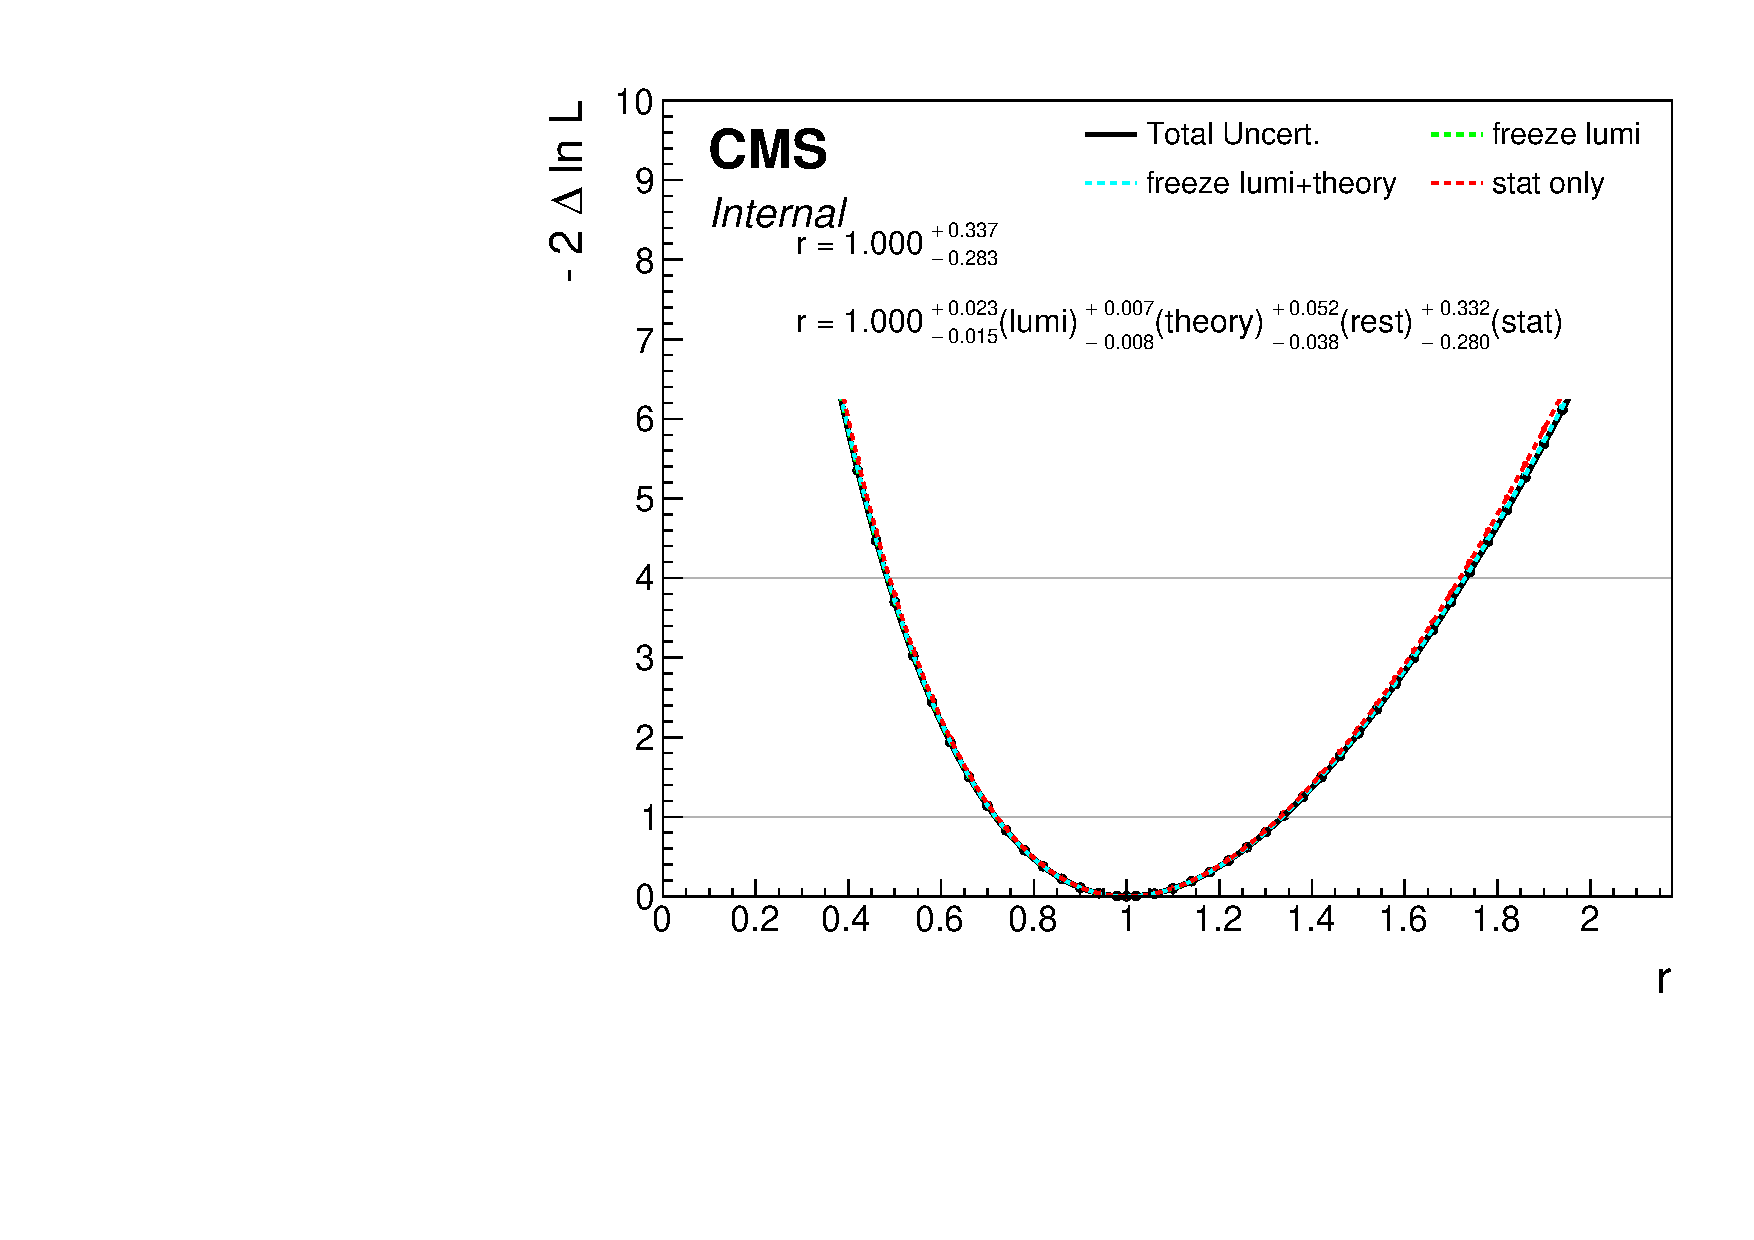
\includegraphics[height=.33\textheight]{scan_expected_Run2_SR4P_phoMC_lepCR_mZZGwp80.pdf}
  \caption{\captionScan{mass of the $\PZ\PZ\PGg$ system}{\texttt{wp80}}{MVA ID}{s}{}}
  \label{fig:scan_Run2_SR4P_phoMC_lepCR_mZZGwp80}
\end{figure}

\begin{figure}
  \centering
  \includegraphics[height=.33\textheight]{Figures/dataMC/Run2/lepCR/SR4P/SYS_wp90pt_central_pow.pdf}
  \hfill
  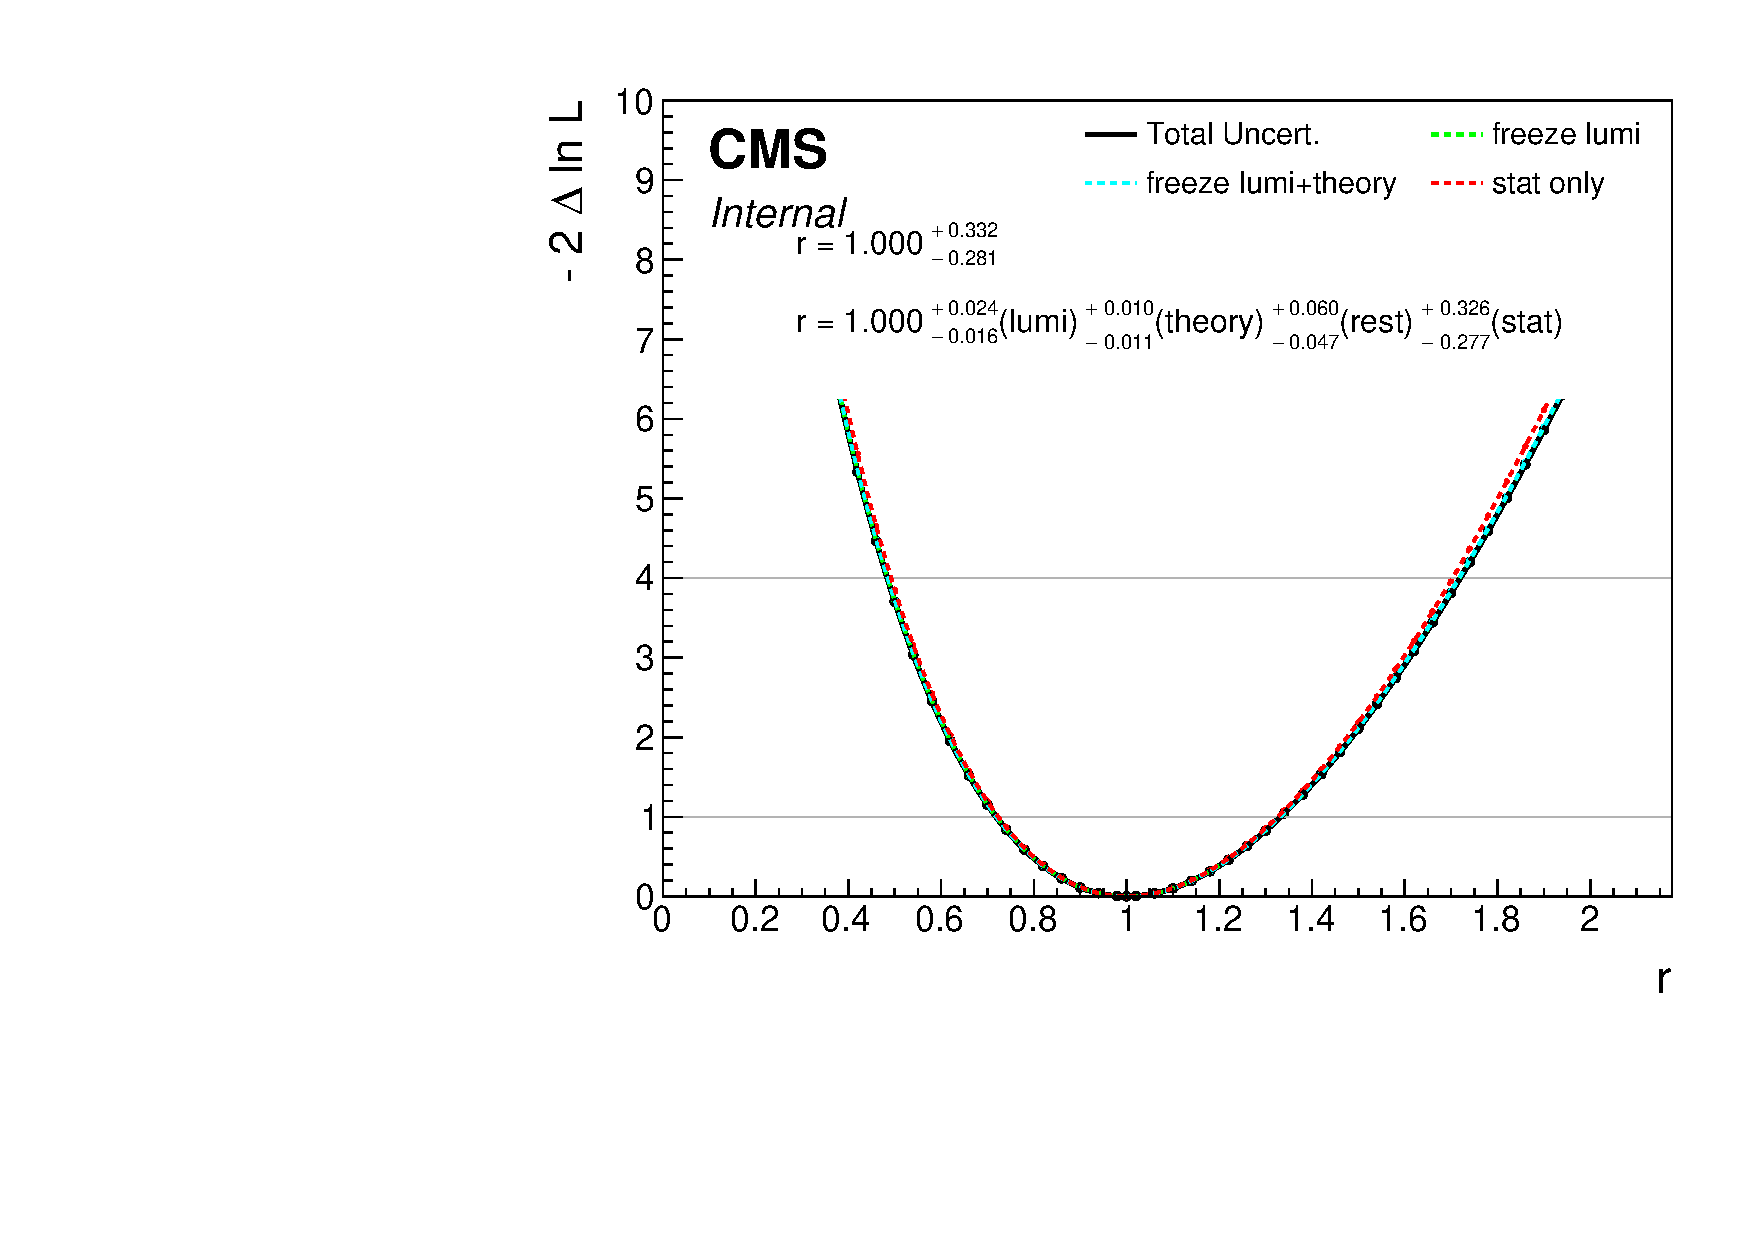
\includegraphics[height=.33\textheight]{scan_expected_Run2_SR4P_phoMC_lepCR_wp90pt.pdf}
  \caption{\captionScan{transverse momentum of the photon}{\texttt{wp90}}{MVA ID}{s}{}}
  \label{fig:scan_Run2_SR4P_phoMC_lepCR_wp90pt}
\end{figure}

\begin{figure}
  \centering
  \includegraphics[height=.33\textheight]{Figures/dataMC/Run2/lepCR/SR4P/SYS_MVAcut_central_pow.pdf}
  \hfill
  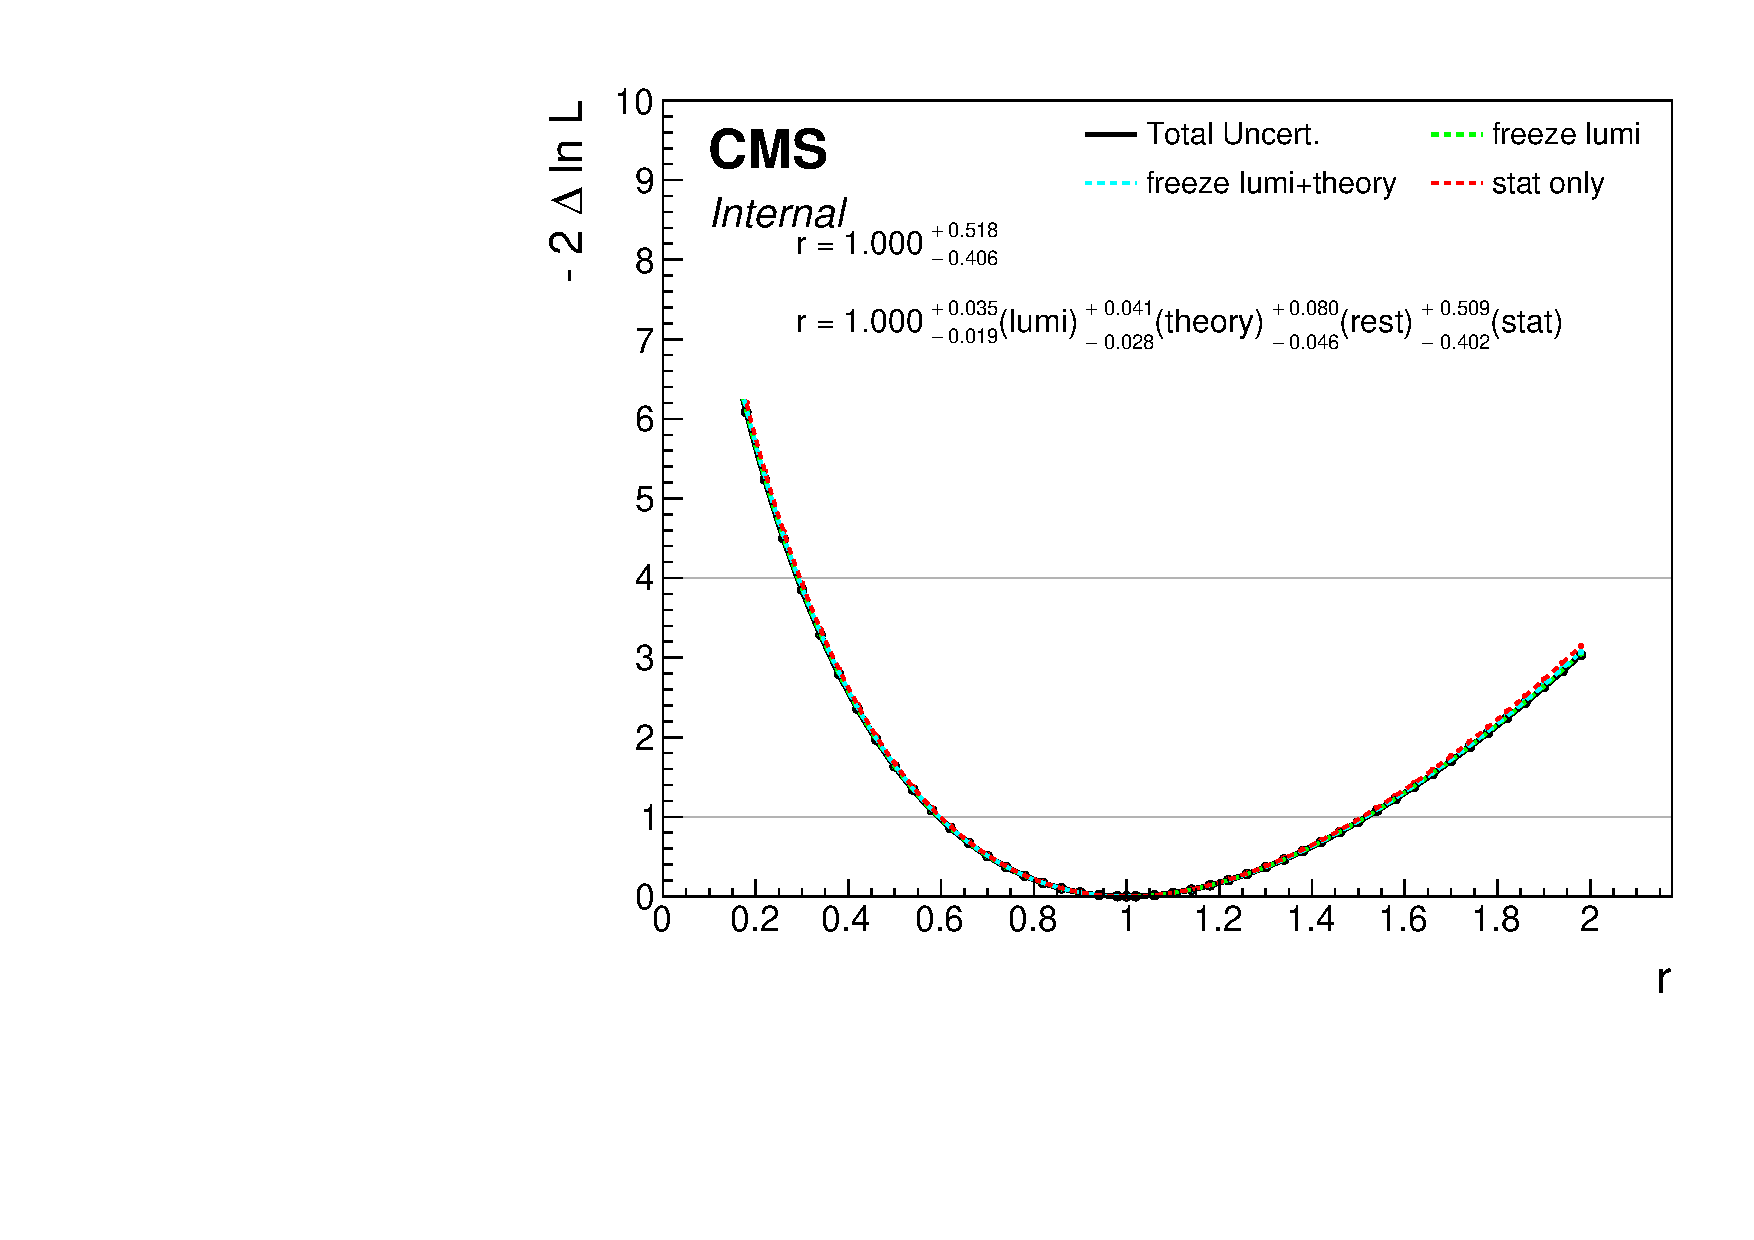
\includegraphics[height=.33\textheight]{scan_expected_Run2_SR4P_phoMC_lepCR_MVAcut.pdf}
  \caption{Likelihood scan for the signal strength parameter
    on the yield in the various bins of the photon MVA ID.
    \descriptionFakePhoton{s}.
    The FSR cut is not applied.
    The effect of groups of nuisance parameters on the uncertainty is assessed by sequentially fixing their value in the fit.
  }
  \label{fig:scan_Run2_SR4P_phoMC_lepCR_MVAcut}
\end{figure}
